\documentclass[preprint,12pt]{elsarticle}

\usepackage{siunitx}
\usepackage{amssymb}

\usepackage{float}
\usepackage{import}
\usepackage{pgf}
\usepackage{graphicx} 
% NOTE required for pgf plots containing underscores in the labels
\usepackage[english]{babel}
\usepackage{underscore}
\usepackage{amsmath}
\usepackage{enumitem}
\usepackage{amsfonts}
\usepackage{caption}
\usepackage{booktabs}
\def\mathdefault#1{#1}
\everymath=\expandafter{\the\everymath\displaystyle}
% \usepackage{fontspec}

\usepackage{adjustbox}

\usepackage{caption}
\usepackage{subcaption}

\usepackage{multirow}


\newcommand{\figurestorepath}{../packages/hvacmarl6e43_notebooks/__datastore__}


\journal{TODO}

\begin{document}

\begin{frontmatter}

%% Title, authors and addresses

%% use the tnoteref command within \title for footnotes;
%% use the tnotetext command for theassociated footnote;
%% use the fnref command within \author or \address for footnotes;
%% use the fntext command for theassociated footnote;
%% use the corref command within \author for corresponding author footnotes;
%% use the cortext command for theassociated footnote;
%% use the ead command for the email address,
%% and the form \ead[url] for the home page:
%% \title{Title\tnoteref{label1}}
%% \tnotetext[label1]{}
%% \author{Name\corref{cor1}\fnref{label2}}
%% \ead{email address}
%% \ead[url]{home page}
%% \fntext[label2]{}
%% \cortext[cor1]{}
%% \affiliation{organization={},
%%             addressline={},
%%             city={},
%%             postcode={},
%%             state={},
%%             country={}}
%% \fntext[label3]{}

\title{TODO Title}

%% use optional labels to link authors explicitly to addresses:
%% \author[label1,label2]{}
%% \affiliation[label1]{organization={},
%%             addressline={},
%%             city={},
%%             postcode={},
%%             state={},
%%             country={}}
%%
%% \affiliation[label2]{organization={},
%%             addressline={},
%%             city={},
%%             postcode={},
%%             state={},
%%             country={}}

\author[inst1]{Author One}

\affiliation[inst1]{organization={Department One},%Department and Organization
            addressline={Address One}, 
            city={City One},
            postcode={00000}, 
            state={State One},
            country={Country One}}

\author[inst2]{Author Two}
\author[inst1,inst2]{Author Three}

\affiliation[inst2]{organization={Department Two},%Department and Organization
            addressline={Address Two}, 
            city={City Two},
            postcode={22222}, 
            state={State Two},
            country={Country Two}}

\begin{abstract}
TODO
\end{abstract}

\begin{graphicalabstract}
%\includegraphics{grabs}
\end{graphicalabstract}

\begin{highlights}
\item Research highlight TODO
\end{highlights}

\begin{keyword}
%% keywords here, in the form: keyword \sep keyword
keyword one \sep keyword two
%% PACS codes here, in the form: \PACS code \sep code
\PACS 0000 \sep 1111
%% MSC codes here, in the form: \MSC code \sep code
%% or \MSC[2008] code \sep code (2000 is the default)
\MSC 0000 \sep 1111
\end{keyword}

\end{frontmatter}

%% \linenumbers

%% main text
\section{Introduction}
Climate change and the energy crisis are challenges that humanity must collectively address.
Many countries have set carbon neutrality targets, as buildings and the construction sector 
account for approximately one-third of global final energy consumption and 15\% of global 
greenhouse gas emissions. Therefore, reducing energy consumption in buildings plays a crucial 
role in achieving carbon neutrality~\cite{ref1}. Among these efforts, effective control and 
efficient operation of HVAC systems in buildings have become a key focus, as these systems 
typically account for 40\% of a building's total energy consumption, with approximately 30\% during 
the operational phase~\cite{ref2, ref3}. Surveys indicate that only 38\% of office occupants are 
satisfied with the thermal comfort of their offices~\cite{ref3}. Consequently, ensuring effective 
control of HVAC systems to reduce energy consumption while maintaining indoor comfort has become a 
critical issue for the health and productivity of office occupants~\cite{ref4, ref7}.

Traditional control methods for HVAC systems rely on rule-based feedback control (RBC), typically 
implemented through PID controllers that adjust temperature setpoints and schedules to change system 
states~\cite{ref5}. Although rule-based methods are easy to implement, they lack the ability to handle 
complex weather variations, potentially leading to suboptimal building performance~\cite{ref6}. 
Model-based control methods, such as Model Predictive Control (MPC), can accurately meet system 
constraints and perform multi-objective optimization~\cite{ref7, ref8}. However, the precise parameters 
of building models vary in real-time due to factors like time and climate, potentially reducing the 
effectiveness of optimized operations. Additionally, MPC requires specific building models, making it 
difficult to generalize across different buildings. Model-based optimization can also be computationally 
intensive when dealing with high-dimensional spaces, making it unsuitable for real-time decision-making, 
which hinders its widespread adoption~\cite{ref9}.

With the proliferation of sensing devices and enhanced computational power, model-free Deep Reinforcement Learning (DRL) 
methods have become increasingly common among researchers for optimizing building thermodynamics. These methods 
have demonstrated progress in handling large state-action spaces~\cite{ref10, ref11} and complex indoor environments~\cite{ref12, ref13, ref14}. 
Despite the extensive application of DRL techniques in previous studies, significant challenges remain in addressing 
multi-zone HVAC control problems with continuous action spaces~\cite{ref15}. In practical applications, multi-zone thermal 
control involves complex control agents that must balance competition and collaboration, further increasing the 
complexity and difficulty of solving the problem~\cite{ref16}. Several studies have applied multi-agent deep reinforcement 
learning (MADRL) to multi-zone thermal control. For example, in \cite{ref17}, Bo et al. proposed 
an HVAC control method based on MATD3 to reduce energy costs while maintaining commercial building room 
temperatures within the desired range. In \cite{ref18}, Li et al. introduced a multi-zone thermal 
control algorithm (MOCA) based on MADRL to maximize energy savings in laboratory settings. In \cite{ref19}, 
Homod et al. proposed a method called Deep Clustering of Cooperative Multi-Agent Reinforcement Learning (DCCMARL) to 
jointly optimize building energy consumption and PMV. In \cite{ref20}, Xue et al. utilized a GA-MADDPG 
approach to optimize building energy consumption by considering regional energy allocation. In \cite{ref21}, 
Abishu et al. presented an MADRL-based energy management algorithm for real-time energy management in smart homes, 
focusing on occupant comfort.
However, these studies have not adequately considered the impact 
of spatial position differences on MADRL model performance, particularly the significant effect of radiant temperature 
on thermal comfort in rooms with varying spatial positions. Differences in thermal comfort due to room 
locations may significantly impact control strategy effectiveness. Therefore, there is an urgent need to 
remodel building environments to more accurately reflect spatial differences. This highlights the necessity 
of developing novel MADRL methods capable of effectively handling the complexities of multi-zone environments 
to optimize control performance.

Meanwhile, another issue cannot be ignored: many DRL algorithms using EnergyPlus for simulation rely on the 
BCVTB platform. Although BCVTB provides a visual interface, it uses EnergyPlus version 8.5.0. Subsequent versions 
have introduced major updates to fix bugs and improve the accuracy of coefficient calculations. Hence, adopting a 
new platform has become an urgent requirement. To address this, this study uses a new platform called Building Gym 
for experiments, which employs EnergyPlus version 23.2.0.

In summary, the main contributions of this paper include:
\begin{enumerate}[label=\arabic*)]
    \item Considering the fuzziness of building thermal dynamics models and the uncertainty of parameters, we formulate a multi-zone HVAC energy management scheme and apply it to a two-story office building model to investigate the effectiveness of the proposed algorithm.
    \item We propose a real-time control algorithm aimed at facilitating effective coordination between room thermal comfort and HVAC energy consumption using a multi-agent deep reinforcement learning (MAPPO) algorithm, further optimized with a Population-Based Training (PBT) approach. This algorithm operates without requiring explicit building thermal dynamics models or the prediction of uncertain parameters.
    \item We implemented a joint simulation environment based on Building Gym for training and testing the proposed algorithm. This environment enables the use of the latest version of EnergyPlus through a simplified EMS interface, reducing discrepancies with real-world scenarios.
\end{enumerate}
\section{Methods}

\subsection{HVAC Operation Model}

This paper considers an HVAC control system consisting of a chiller, AHU, and VAV. When turned on, it adjusts the overall output power of the HVAC based on external temperature variations and other factors. The operation mode $\sigma_t$ can be described as follows:

\begin{equation} \label{eq:hvac-op}
    \sigma_t = 
    \begin{cases} 
        \zeta_{\text{hvac},t}, & \text{if } N_{\text{occ},t} \neq 0 \\
        0, & \text{if } N_{\text{occ},t} = 0 
    \end{cases}
\end{equation}

In Equation~\ref{eq:hvac-op}, $\zeta_{\text{hvac},t}$ represents the power factor of the HVAC at time $t$, 
a value between 0 and 1 that changes depending on environmental factors. $\sigma_t = \zeta_{\text{hvac},t}$ 
indicates that the HVAC is operational at time $t$, while $\sigma_t = 0$ indicates that the HVAC is off.
 $N_{\text{occ},t}$ denotes the occupancy index of the office space at time $t$.

When the HVAC system is operational, $T_{\text{set},t}^{\min}$ and $T_{\text{set},t}^{\max}$ 
represent the minimum and maximum setpoints of the control zone. The control zone setting is continuous, 
meaning the setpoint $T_{\text{set},t}$ can be chosen within the range:
\begin{equation}
T_{\text{set},t} \in \left[ T_{\text{set},t}^{\min}, T_{\text{set},t}^{\max} \right]
\end{equation}

\subsection{Energy Consumption Model}

The energy consumption model in this paper refers to the HVAC energy consumption of an 
entire building, which aligns with real-world settings since an HVAC system can control 
the states of multiple rooms, and its energy consumption is an aggregate of multiple rooms. 
The energy consumption of the HVAC system mainly consists of three components: the energy 
consumption of the cooling tower, the AHU, and the VAV. Let $\Delta T$ denote the timestep. 
$P_{\text{hvac}}, P_{\text{coolingtower}}, P_{\text{ahu}},$ and $P_{\text{vav}}$ represent 
the power levels of the HVAC system, cooling tower, AHU, and VAV, respectively, and $\zeta_{\text{coolingtower}}, 
\zeta_{\text{ahu}}, \zeta_{\text{vav}}$ represent their corresponding power factors.

The actual power of the HVAC system can be calculated as follows:
\begin{equation}
P_{\text{hvac}}\zeta_{\text{hvac},t} = P_{\text{coolingtower}} \zeta_{\text{coolingtower},t} + P_{\text{ahu}} \zeta_{\text{ahu},t} + P_{\text{vav}} \zeta_{\text{vav},t}
\end{equation}

Then, the energy consumption of the HVAC system within a timestep can be calculated as follows:
\begin{equation}
E_{\text{hvac},t} = \Delta T P_{\text{hvac}} \zeta_{\text{hvac},t}
\end{equation}

\subsection{PMV Model}

The thermal comfort model adopted in this paper is based on the internationally 
recognized ASHRAE-55 thermal comfort model. The calculation depends on indoor dry bulb 
temperature, indoor radiant temperature, humidity, air velocity, and the clothing insulation 
of office occupants. Since this paper primarily focuses on controlling indoor temperature setpoints, 
certain assumptions and simplifications have been made to the PMV model. The simplified thermal comfort $\text{PMV}_t$ 
is described as follows:

\begin{equation} \label{eq:pmv}
    \begin{gathered}
        \text{PMV}_t = \text{PMV}(T_{\text{drybulb},t}, T_{\text{radiant},t}, \text{RH}_t, v_t) \\
        v_t = 
        \begin{cases} 
            v_{\text{air},t} = 0.1 \, \text{m/s}, & \text{for } t \in [0, 24\text{hr}] \\
            \text{CLO}_t = 0.5, & 
        \end{cases}
    \end{gathered}
\end{equation}

In Equation~\ref{eq:pmv}, $\text{PMV}_t$ represents the PMV value of a room at time $t$, 
while $T_{\text{drybulb},t}$, $T_{\text{radiant},t}$, and $\text{RH}_t$ represent the 
indoor dry bulb temperature, indoor radiant temperature, and humidity at time $t$, respectively.
 $v_t$ represents the air velocity at time $t$, which is assumed to be 0.1 m/s. The clothing 
 insulation of office occupants, $\text{CLO}_t$, is assumed to be 0.5, representing typical summer attire.

At the same time, $\text{PMV}_t$ is simplified to remain within the comfort range, 
and therefore must satisfy the following constraint:

\begin{equation}
    \text{PMV}^{\min} \leq \text{PMV}_t \leq \text{PMV}^{\max}
\end{equation}

\subsection{Reward Function Design}

The design of the reward function can be used to measure whether an agent's actions contribute 
to the optimization of the overall problem. Generally, it is a continuous numerical signal, 
where higher reward values indicate that the agent's actions are moving toward more beneficial optimization, 
and vice versa. Since agents have both cooperative and competitive relationships, the reward design must 
incorporate multiple dynamic factors to better balance comfort and energy consumption optimization.

To achieve this, a reward mapping space is designed to enable the optimization of PMV and HVAC energy consumption. 
Using a unified approach, PMV is first normalized into the interval to express the deviation of PMV 
from the ideal value (PMV = 0). HVAC energy consumption is then similarly normalized. Finally, the state $s_t^m$ 
is mapped into a reward space $p_{x,y}^m$, where the location is defined as:

\begin{equation}
    \begin{gathered}
        x = 0.5 - |\text{PMV}| / 0.5, \quad 0 \leq x \leq 1 \\
        y = (P_{\text{hvac},t} - P_{\text{hvac}}^{\min}) / (P_{\text{hvac}}^{\max} - P_{\text{hvac}}^{\min}), \quad 0 \leq y \leq 1
    \end{gathered}
\end{equation}

The reward depends on the state $s_t^m$ and the position difference between $s_t^m$ 
and $s_{t-1}^m$ in the reward space. This produces a directional vector pointing from $s_{t-1}^m$ 
to $s_t^m$, defined as follows:

\begin{equation}
    r_t^m = r_{\text{distance}}^m \cdot r_{\text{angle}}^m
\end{equation}

where:

\begin{equation}
    \begin{gathered}
        r_{\text{distance},t}^m = \sqrt{(p_{x,t}^m - p_{x,t-1}^m)^2 + (p_{y,t}^m - p_{y,t-1}^m)^2} \\
        r_{\text{angle},t}^m = \arctan\left(\frac{p_{y,t}^m - p_{y,t-1}^m}{p_{x,t}^m - p_{x,t-1}^m}\right)
    \end{gathered}
\end{equation}


\subsection{PMV-Energy Consumption Joint Optimization Problem}

Based on the operational constraints and related requirements mentioned above, this section 
formulates the joint optimization problem of controlling the cooling setpoint in the environment to 
achieve both the optimal PMV and the lowest HVAC energy consumption, as follows:

\begin{equation}
\min \sum_{t} \lambda E_{\text{hvac},t} + (1 - \lambda) |\text{PMV}_t|
\end{equation}

In the equation above, $t$ represents the time interval, and $\lambda$ represents the 
weighting factor for balancing uncertain parameters. If the dynamics of the environment are 
known (e.g., the probabilistic distribution of operations), model-based predictive control can be 
used to solve this problem. However, given the presence of indoor temperature and other associated states, 
it is challenging to develop an efficient and effective warm-up control model using traditional modeling techniques. 
Therefore, it is necessary to reformulate the control problem as a multi-agent reinforcement learning problem 
to describe the relationships of competition and cooperation among multiple agents. Let $N$ represent the 
number of independent agents. To solve the problem as a multi-agent Markov game, this problem is first decomposed 
into three main components: states, actions, and rewards, denoted as $S, A, R$, where $s \in S$, $a \in A$, 
and $r \in R$. $S$ represents the environmental state, and each agent updates its 
state-action function $V^\pi(o, a)$ (where $\pi$ is the policy network’s weight parameter) based 
on the observations of the environment.

The dynamic information obtained locally is $o = (o_1, o_2, \ldots, o_N)$, which corresponds to 
actions $a = (a_1, a_2, \ldots, a_N)$. At the end of all actions, rewards and new states are returned by the environment.
Let $t = \{1, 2, \ldots, T\}$ represent the time intervals within the simulation, 
and let $m = \{1, 2, \ldots, M\}$ represent the different zones of the building. $M$ has a 
maximum value of 8. For a certain time $t$ in a zone $m$, its state is denoted as $s_t^m$, 
and $T_{\text{set},t}^m$ represents the setpoint value in zone $m$ at time $t$. The state of 
each agent consists of the indoor zone state and the HVAC operating state, which include indoor dry bulb temperature, 
indoor radiant temperature, humidity, occupancy, air velocity, and clothing insulation of the occupants. 
The HVAC energy consumption is determined by these states. Note that this study does not use directly 
observed thermal comfort indices (e.g., PMV/PPD), but rather approximates the relationship between those 
indices and their classification. This approach aligns with practical implementations where intelligent agents 
receive observation data indirectly. Agents generate actions based on observations, which are input into the 
neural network to calculate spatial temperature predictions and generate corresponding control strategies.

Let $\mathbf{s}_{t,a}$ represent all zone states at time $t$, including zone 
states and HVAC states, and the action $\mathbf{a}_t$ is:

\begin{equation}
(\mathbf{s}_{t,a}) = \{s_1^1, s_1^2, \ldots, s_T^M\}, (\mathbf{a}_t) = \{a_1^1, a_2^1, \ldots, a_m^M\}
\end{equation}

\section{MAPPO Control Algorithm Design}

This section proposes a control algorithm based on MAPPO to address the aforementioned 
joint optimization problem. MAPPO significantly enhances the capability of PPO 
by introducing adaptability mechanisms tailored for multi-agent scenarios. As an online 
policy learning method, PPO excels in dynamically and rapidly fine-tuning its strategy in 
real time based on interactions with the environment. This continuous adjustment is 
particularly beneficial in BES (Building Energy Simulation) environments, where system 
dynamics or external factors (such as weather conditions or occupancy patterns) tend to change 
rapidly~\cite{ref22}. This strategy enables continuous evaluation of the overall state, 
allowing for quick responses to system changes and reducing risks associated with sudden disruptions. 
Therefore, this study adopts PPO to train the algorithm framework, as shown in Figure2. 
In this framework, each agent in the multi-agent system interacts with its respective environment 
through Building Gym, obtaining data and providing specific control actions as feedback.

PPO is derived from a simplified version of the TRPO algorithm. In PPO, each agent incorporates a 
clipped objective to ensure stable updates. The PPO objective function is defined as follows:

\begin{equation}
L^{\text{CLIP}}(\theta) = \mathbb{E}_t \left[ \min \left( \mu_\theta(A), \, \text{clip}(\mu_\theta(A), 1 - \epsilon, 1 + \epsilon) A_t \right) \right]
\end{equation}

Here, $\mathbb{E}_t$ represents the expectation over time steps, 
and $\mu_\theta(A) = \pi_{\theta,\text{new}}(a_t | s_t) / \pi_{\theta,\text{old}}(a_t | s_t)$
 denotes the ratio of the new policy to the old policy. $\epsilon$ is the clipping factor, 
 which limits the magnitude of policy updates to avoid excessively large changes. 
 $\hat{A}$ represents the generalized advantage estimator (GAE), used to evaluate the 
 advantage of taking an action under a given state. It is computed as follows:

\begin{equation}
\hat{A}(t) \approx r(s, a) + \gamma V_\phi(s_{t+1}) - V_\phi(s_t)
\end{equation}

The critic network is parameterized by $\phi$ and is learned using gradient descent with the following loss function:

\begin{equation}
L^{\text{VF}}(\phi) = \mathbb{E}_t \left[ (V_\phi(s_t) - (r_t + \gamma V_\phi(s_{t+1})))^2 \right]
\end{equation}

PPO combines the policy loss, value loss, and entropy bonus $\Omega[\pi_\theta]$ to enhance exploration. 
The total loss function is:
\begin{equation}
L(\theta) = \mathbb{E}_t \left[ L^{\text{CLIP}}(\theta) - c_1 L^{\text{VF}}(\phi) + c_2 \Omega[\pi_\theta](s_t) \right]
\end{equation}
Here, $c_1$ and $c_2$ are constants, and $\Omega[\pi_\theta]$ is the entropy term, 
which provides regularization for the policy.

In Figure 2, the MAPPO framework includes the environment and multiple agents, where the controller for 
each room acts as an agent executing the PPO algorithm. Each PPO agent has both an action network and a 
critic network. The MAPPO framework uses a centralized training and decentralized execution paradigm, allowing 
agents to share the global value function during training while independently observing and acting during execution. 
The training process adopts a centralized method by integrating observations and actions to derive policies. 
During execution, only local observations are used for random exploration. Below, taking an agent as an example, 
we detail how centralized training is performed in the MAPPO framework and explain the model-based approach for policy learning.
In the centralized training phase, the critic network evaluates the global state-value function:

\begin{equation}
V^\pi(s, a_1, a_2, \ldots, a_N \mid \phi), \quad \text{where } s = (s_1, s_2, \ldots, s_N),
\end{equation}

and $\phi$ is the parameter of the critic network. The critic network uses this function to evaluate the policy. 
The loss function for the critic network is minimized as follows:

\begin{equation}
\theta_{\text{loss}}^\phi = \mathbb{E}\Bigl[\bigl(V^\pi(s', a_1', a_2', \ldots, a_N' \mid \phi') - V^\pi(s, a_1, a_2, \ldots, a_N \mid \phi)\bigr)^2\Bigr],
\end{equation}

where $s'$ and $a'$ are the updated states and actions. The critic network updates its parameters based on the 
gradient direction $\nabla_\phi$. The global state information $s = (s_1, s_2, \ldots, s_N)$ is collected to
 adjust the parameters of the critic network.

The actor network assumes a global value function by integrating the global state and outputs actions:

\begin{equation}
a = (a_1, a_2, \ldots, a_N).
\end{equation}

By introducing such a centralized value function, the global state can be integrated, and the partially 
observable Markov Decision Process (MDP) is fully converted into an observable MDP. This approach improves 
the learning process for the value function while enhancing training efficiency and speed. The corresponding 
gradient formula is as follows:

\begin{equation}
\nabla_\theta J = \mathbb{E}\bigl[\nabla_\theta Q(s, a_1, a_2, \ldots, a_N \mid \phi) \nabla_\theta \pi(s \mid \theta)\bigr].
\end{equation}

In the decentralized execution phase, each actor only makes local observations and decisions 
based on local sensors. This process eliminates the need for global broadcasting and reduces computational 
and communication overhead. By efficiently utilizing parameterized policy functions, each agent does not 
require information from other agents to approximate the globally optimal actions.
\subsection{Population-Based Training (PBT)}

\begin{figure}
    \centering
    \adjustbox{max width=\textwidth, max height=0.8\textheight}{
        \includegraphics{figures/PBT.png}
    }
\end{figure}

Population-Based Training (PBT) is an adaptive optimization method that combines 
hyperparameter optimization and model training, commonly used in deep learning and 
reinforcement learning tasks. It maintains a population of models and their corresponding 
hyperparameters, dynamically adjusting the hyperparameters and model weights to improve 
training efficiency and final performance~\cite{ref23}.

\section{Testbed and Simulation Environment}

Figure 1 illustrates the internal structure of BuildingGym, which consists of two main modules: 
the built-in EnergyPlus module and the AI algorithm module.

The EnergyPlus module leverages the EnergyPlus-OOEP module within BuildingGym in combination with 
EnergyPlus to perform precise simulations, facilitating realistic modeling of building dynamics and 
HVAC energy consumption. Compared to the widely used Building Control Virtual Test Bed (BCVTB) platform, 
this module offers the advantage of utilizing EnergyPlus version 23.2, which is a significant upgrade 
from the EnergyPlus 8.5.0 version employed by BCVTB. This updated version addresses numerous bugs and numerical 
calculation issues present in older versions of EnergyPlus, making it more suitable for accurate simulations.

The AI algorithm module is constructed using the RLlib library, a specialized open-source framework designed 
explicitly for reinforcement learning applications. RLlib provides a comprehensive suite of state-of-the-art 
algorithms and optimization techniques, facilitating the seamless development of experimental setups and 
enabling robust evaluation of model performance. Its modular architecture and extensive documentation support 
efficient experimentation, reproducibility, and the benchmarking of reinforcement learning methods in diverse environments.
TODO
\begin{figure}
    \centering
    \adjustbox{max width=\textwidth, max height=0.8\textheight}{
        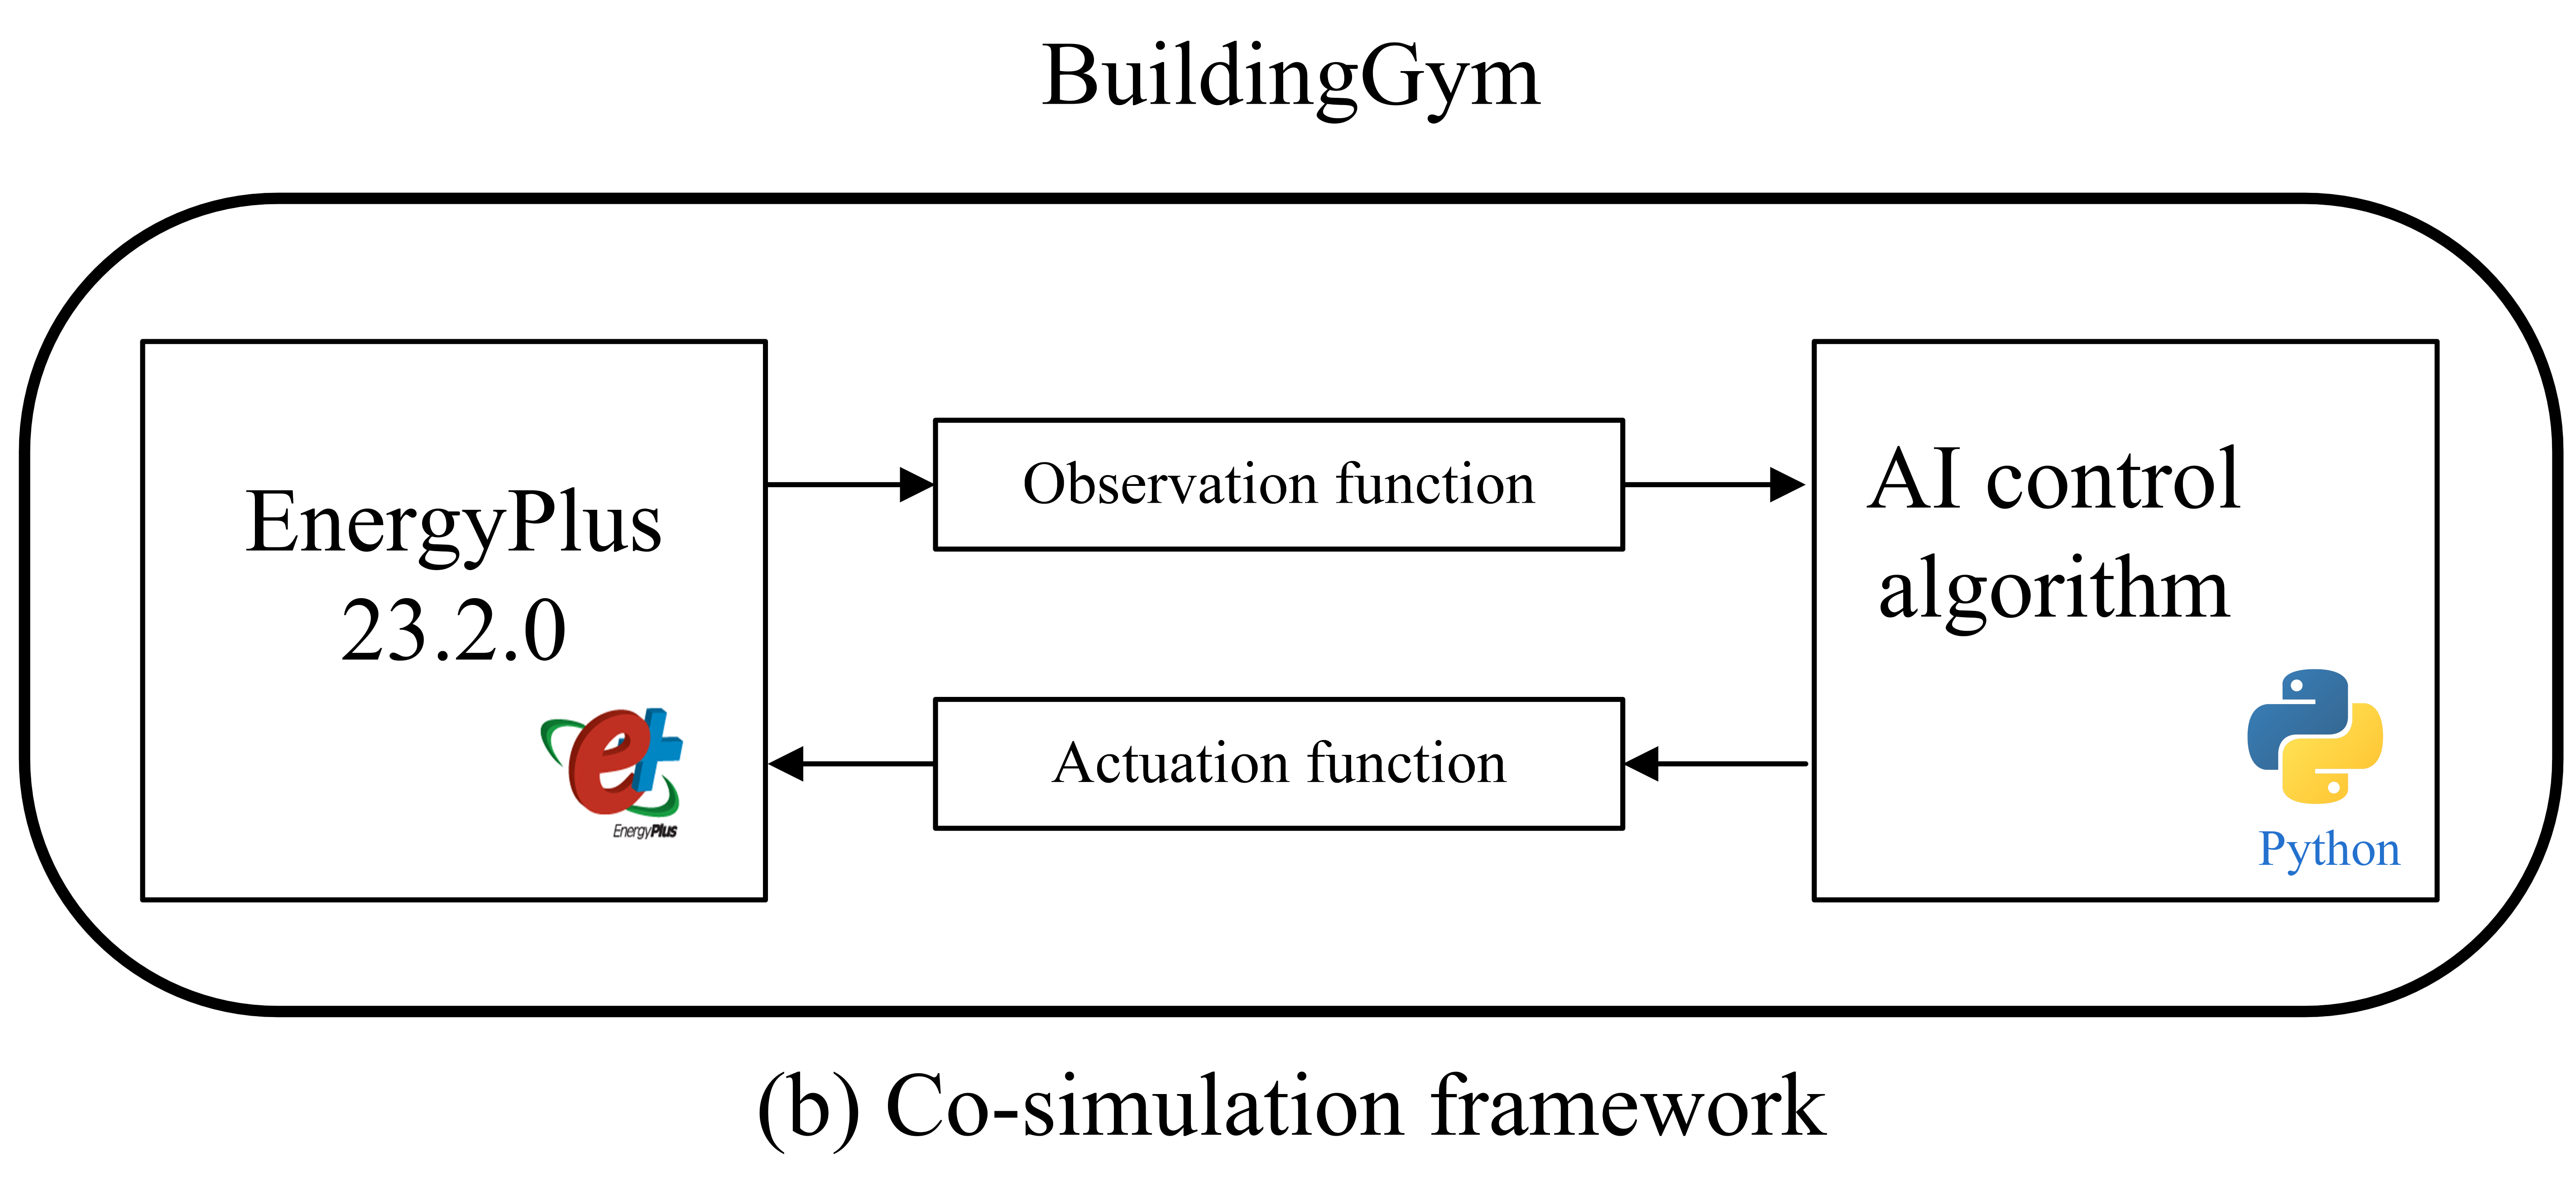
\includegraphics{figures/buildinggym.png}
    }
\end{figure}

\subsection{Building model}

\begin{figure}[htbp]
    \centering
    \begin{subfigure}[b]{0.3\textwidth}
        \centering
        \includegraphics[width=\textwidth]{figures/figure:building.png}
        \caption{Building, Whole}
    \end{subfigure}
    \begin{subfigure}[b]{0.3\textwidth}
        \centering
        \includegraphics[width=\textwidth]{figures/figure:building-f1.png}
        \caption{Building, 1st Floor}
    \end{subfigure}
    \begin{subfigure}[b]{0.3\textwidth}
        \centering
        \includegraphics[width=\textwidth]{figures/figure:building-f2.png}
        \caption{Building, 2nd Floor}
    \end{subfigure}
\end{figure}



% In the simulation conducted in this study, as shown in Figure 2, the RL algorithm 
% primarily controls the simulation environment within EnergyPlus through EnergyPlus-OOEP. 
% At the end of each "runperiod: timestep calling point" event, 
% EnergyPlus-OOEP interacts with the EnergyPlus environment by retrieving information 
% from the observation space and applying computed values from the action space to 
% control the zone mean air temperature setpoint in EnergyPlus. 
% The reward is calculated internally by EnergyPlus-OOEP to evaluate the quality of the actions (TODO WRONG!!!).

The target building model used in this study was constructed in DesignBuilder 
and represents a two-story medium-sized office building. 
The building has a total of eight rooms, each with windows on all elevations 
except for the portion of the building's interior wall, totaling seven windows per room, 
with glass doors on the building's interior wall. The HVAC system in the building 
includes a cooling tower, a chiller, a boiler, and a VAV system. 
The building operates daily from 7:00 a.m. to 6:00 p.m. except weekends.
To meet the testing requirements, the indoor temperature during building occupancy 
is set at \SI{23}{\celsius} and \SI{24}{\celsius}.
The PMV average value and average energy consumption are calculated 
separately for each temperature setting to ensure that the baseline energy consumption 
and PMV optimal points can be identified. 
The training of the RL agents is conducted from July 1 to July 31, 
with a time step interval of 10 minutes. 
TODO The weather file used for training is \texttt{SGP_Singapore_486980_IWEC.epw}.
The HVAC parameters are listed in Table 3. 
\begin{table}[h!]
\centering
\caption{HVAC parameters.}
\begin{tabular}{@{}llc@{}}
\toprule
\textbf{Feature} & \textbf{Parameters} & \textbf{Setting} \\ \midrule
\multirow{2}{*}{\textbf{General}} 
    & High-Speed/Low-Speed Sensible Heat Ratio & 0.75 \\
    & Nominal Capacity (W) & 3500 \\ \midrule
\multirow{2}{*}{\textbf{Cooling}} 
    & Rated Cooling COP (W/W) & 3.0 \\
    & Internal Static Air Pressure (Pa) & 450 \\ \midrule
\multirow{4}{*}{\textbf{Heating}} 
    & Burner Efficiency & 0.98 \\
    & Nominal Capacity (W) & 3500 \\
    & Fan Total Efficiency & 0.7 \\
    & Pressure Rise (Pa) & 600 \\ \midrule
\multirow{4}{*}{\textbf{Fan}} 
    & Maximum Flow Rate (m\textsuperscript{3}/s) & 3.0 \\
    & Power Minimum Flow Fraction & 0.25 \\
    & Motor Efficiency & 0.9 \\
    & Motor In Air-stream Fraction & 1.0 \\ \bottomrule
\end{tabular}
\label{table:hvac_parameters}
\end{table}


\section{Experiment}

All algorithms were computed on the same machine using the same platform 
to ensure a fair comparison among the algorithms. 

\begin{figure}[H]
    \caption{TODO}
    \centering
    \begin{itemize}
        \item Hardware
            \begin{description}
                \item[RAM] 64 GiB Mem / 975MiB Swap
                \item[CPU] AMD Ryzen 9 5950X 16-Core Processor
                \item[GPU] NVIDIA GeForce RTX 4070 Ti
            \end{description}
        \item Software
            \begin{description}
                \item[OS] \texttt{Debian 6.1.115-1 (2024-11-01) x86_64 GNU/Linux}
                \item[Python] \texttt{3.11}
                \item[EnergyPlus] TODO
                \item[PyTorch] TODO
            \end{description}
    \end{itemize}
\end{figure}


\section{Results and Discussion}

\subsection{TODO}

TODO

\subsection{Overall Performance}

\begin{figure}[H]
    \centering
    \adjustbox{max width=\textwidth}{
        \subimport{\figurestorepath}{figure:avg-elec-pmv-abs-mean.pgf}
    }
    \caption{TODO.}
\end{figure}

\begin{figure}[H]
    \centering
    \adjustbox{max width=\textwidth}{
        \subimport{\figurestorepath}{figure:elec-v-pmv-abs-rolling.pgf}
    }
    \caption{Power consumption vs absolute PMV for different control strategies.}
\end{figure}

\begin{figure}[H]
    \centering
    \adjustbox{max width=\textwidth}{
        \subimport{\figurestorepath}{figure:elec-mean-v-pmv-abs-mean.pgf}
    }
    \caption{TODO.}
\end{figure}

This section provides a general assessment of the simulation results of three methods, 
namely the rule-based method, PPO, and MAPPO. These algorithms are applied to the models mentioned above. 
In this paper, the PMV at each moment in time is treated as an absolute value, 
so that an absolute value of PMV close to 0 indicates that the algorithm is more effective in controlling the room comfort. 
In order to be able to compare the different control strategies in a complete way, 
in Fig. 1, the strategies under different temperature control ranges are tested in this section, 
including the baseline strategy and the two reinforcement learning strategies, PPO and MAPPO. 
The temperature control range of the baseline strategy is set from 22.\SI{0}{\celsius} to 24.\SI{5}{\celsius}, with an interval of 0.\SI{5}{\celsius}; 
the PPO and MAPPO strategies are tested in four temperature ranges for optimization, 
which are \SI{20}{\celsius} to \SI{22}{\celsius}, \SI{22}{\celsius} to \SI{24}{\celsius}, \SI{24}{\celsius} to \SI{26}{\celsius} for the local search range, 
and \SI{20}{\celsius} to \SI{30}{\celsius} for the global search range. 

In Fig. 1, it can be clearly seen that compared to the baseline curve, 
the PPO curve as well as the MAPPO curve can reduce the energy consumption to a certain extent for the same absolute value of PMV. 
At the same time, at the same energy consumption, the absolute value of PMV of the MAPPO is lower compared to that of the PPO, 
which indicates that the control of the MAPPO is superior to that of the PPO. 

When comparing PPO and MAPPO in the global search range of \SI{20}{\celsius} to \SI{30}{\celsius}, 
it can be found that the optimal point found by PPO is located near \SI{24}{\celsius} of the baseline, 
while MAPPO is located near \SI{23}{\celsius} of the baseline, 
which highlights the difference between the two strategies in searching for the optimal point. 
At the same time, the optimal point of PPO is closer to the baseline strategy, 
while the optimal point of MAPPO not only achieves the same energy consumption, 
but also achieves a lower absolute PMV, indicating that MAPPO has better control than PPO. 
MAPPO's optimal point not only achieves a lower absolute PMV value compared to the baseline, 
but also its energy consumption is lower, indicating MAPPO's advantage in multi-room control. 

Fig. 2 illustrates the link between absolute PMV values and energy consumption when using different strategies 
to show the difference in performance in terms of control stability and energy optimization between different strategies. 
The line in the figure represents the calculated mean value of the sliding window under the same strategy, 
while the shaded portion of the figure indicates the fluctuation range of the calculated results of the sliding window, 
i.e., the interval of the maximum and minimum values of the strategy under the sliding window, 
which reflects the distribution interval of the results of the strategy within the sliding window. 

The shaded portion of the Single-Agent PPO is larger when it has the same energy consumption, 
which indicates that the PMV fluctuates more in absolute value, demonstrating its poor stability for the control of multiple room temperatures. 
At the same time, the PMV is higher in the part of elec greater than 10M, 
which corresponds to the high-load part of the HVAC work, 
which reflects that the strategy fails to balance energy consumption and thermal comfort effectively, 
especially in the high-load area, and the performance is poor. 

The Baseline strategy selects the cooling setpoint of \SI{23}{\celsius} and \SI{24}{\celsius} as the samples. 
The sample of \SI{23}{\celsius} shows a relatively low absolute value of PMV, and the fluctuation range is smaller than PPO, 
which shows better control stability and thermal comfort, 
while the sample at \SI{24}{\celsius} shows a higher absolute value of PMV, the fluctuation range is smaller than PPO. 

The absolute value of PMV of the MAPPO strategy is lower than the rest of the strategies, 
and the range of fluctuation is smaller, and the curve is smoother with no obvious ups and downs, 
which shows the control stability and the balance of energy consumption and thermal comfort, 
especially in high-load areas. The MAPPO strategy demonstrates control stability 
and the ability to optimize the balance between energy consumption and comfort.


\subsection{Typical Days Comparison}

This section presents the control performance results for a hot summer week (July 19--25) using different control strategies over the course of the week. 
The baseline strategy selected for comparison in this section utilizes temperature setpoints derived from the optimal PMV points obtained from the baseline strategy curves in the previous section, specifically \SI{23.0}{\celsius} and \SI{24.0}{\celsius}. 
The same incentive structures and configurations as above are applied for PPO and MAPPO. 

Figure~2 illustrates a comparison of the average PMV within the building across the different control strategies during the selected week, alongside the baseline control. 
Among these strategies, it is observed that PPO exhibits greater fluctuations and higher average PMV in absolute terms, indicating that PPO's control is less stable for medium-sized buildings with multiple rooms. 
In contrast, both MAPPO and the baseline strategy demonstrate more stable control, with both capable of maintaining PMV below 0.5 throughout periods when the office occupancy index is non-zero. 
During the midday to afternoon hours, the baseline strategy is able to maintain the average PMV at approximately 0.1 in absolute terms, while MAPPO further improves performance, achieving an average PMV close to 0.05 in absolute terms. 
This highlights MAPPO superior ability to control average PMV compared to the other two strategies. 
Additionally, it is evident that the two reinforcement learning (RL) methods decrease the average PMV more rapidly during morning hours when the office occupancy index increases sharply. 
This demonstrates that RL-based methods exhibit greater flexibility in handling complex situations compared to the baseline method.

Figure 3 (TODO) provides a comparison of in-building HVAC energy consumption across the different control strategies over the same week. 
As anticipated, the single-agent PPO strategy consumes relatively low HVAC energy due to its control of the average PMV absolute value at a higher level. 
When comparing the baseline strategy and MAPPO, MAPPO consistently consumes less energy than the baseline during periods when the office occupancy index is non-zero. 
Notably, in the mornings when HVAC energy consumption increases most rapidly, the MAPPO strategy reduces energy consumption by an average of \SI{10}{\percent} compared to the baseline. 
These findings indicate that the MAPPO strategy is not only effective in optimizing energy costs but also enhances thermal comfort. 
This underscores MAPPO's capacity to provide a more adaptive and efficient HVAC control method, achieving the dual objectives of energy savings and improved occupant comfort.

\subsection{Analysis of Control Strategies Across Zones}

\begin{figure}[H]
    \label{figure:time-v-pmv-abs}
    \centering
    \adjustbox{max width=\textwidth}{
        \subimport{\figurestorepath}{figure:time-v-pmv-abs.pgf}
    }
    \caption{TODO.}
\end{figure}

Figure~\ref{figure:time-v-pmv-abs} shows the simulation results for the individual zones
over a period of three days, containing information on the absolute value of the PMV, 
the cooling setpoint for the HVAC, and the upper and lower comfort bounds for the PMV (TODO mv to caption!). 
These zones are located on floors 0F and 1F on one side of the building and are intended 
to provide an in-depth analysis of the differences in the strategies used by the three methods. 
Although the rule-based strategy appears to be very stable in terms of control, 
it can only maintain a setpoint of \SI{23}{\celsius}, which has a limited control range 
and is not conducive to dynamic adjustment. 
The single-agent strategy, on the other hand, exhibits consistent control behavior in all zones. 
However, due to the significant differences in the characteristics of each room within 
a two-story, multi-room building, it is difficult for a single strategy to optimize control 
for the specific needs of each room. This lack of targeting limitation is the main reason 
for the ineffectiveness of single-agent control. 
In contrast, the multi-agent strategy is able to adopt adaptive control behaviors tailored 
to the unique needs of each zone, and thus its overall control effectiveness is superior to 
that of the single-agent strategy. This can be concluded by looking at the HVAC cooling setpoint.

\subsection{Comparison of Discomfort Periods}

\begin{figure}[H]
    \centering
    \adjustbox{max width=\textwidth}{
        \subimport{\figurestorepath}{figure:time-v-comfort.pgf}
    }
    \caption{TODO.}
\end{figure}

Figure 6 (TODO) clearly illustrates the differences between the baseline strategy, the PPO strategy, and the MAPPO strategy. 
Under the baseline strategy with temperature setpoints at \SI{23.0}{\celsius} and \SI{24.0}{\celsius}, 
the absolute PMV values during the morning hours (7 - 9) are relatively high, indicating a more pronounced sense of discomfort during this period. 
Although the PPO strategy significantly reduces discomfort compared to the baseline strategy during the early morning hours, 
it exhibits greater variability and lower stability during the high-load afternoon hours (13--18). 
In contrast, the MAPPO strategy demonstrates superior performance across all time periods, 
maintaining stable control even during peak discomfort periods. 
This indicates that MAPPO provides a more stable and adaptable control strategy, 
effectively balancing thermal comfort and energy efficiency.


%% The Appendices part is started with the command \appendix;
%% appendix sections are then done as normal sections
\appendix

\section{Sample Appendix Section}
\label{sec:sample:appendix}
TODO section %\ref{sec:sample1}
%% If you have bibdatabase file and want bibtex to generate the
%% bibitems, please use
%%
%  \bibliographystyle{elsarticle-num} 
%  \bibliography{cas-refs}

%% else use the following coding to input the bibitems directly in the
%% TeX file.

\begin{thebibliography}{16}

\bibitem{ref1}
Zhang, Yan, et al. "Data-driven estimation of building energy consumption and GHG emissions using explainable artificial intelligence." \textit{Energy}, vol. 262, 2023, p. 125468.
    
\bibitem{ref2}
Wu, Ziyan, et al. "Reinforcement learning in building controls: A comparative study of algorithms considering model availability and policy representation." \textit{Journal of Building Engineering}, vol. 90, 2024, p. 109497.
    
\bibitem{ref3}
Yu, Liang, et al. "Energy-efficient personalized thermal comfort control in office buildings based on multi-agent deep reinforcement learning." \textit{Building and Environment}, vol. 223, 2022, p. 109458.
    
\bibitem{ref4}
Yu, Liang, et al. "A review of deep reinforcement learning for smart building energy management." \textit{IEEE Internet of Things Journal}, vol. 8, no. 15, 2021, pp. 12046–12063.
    
\bibitem{ref5}
DAfram, Abdul, and Farrokh Janabi-Sharifi. "Theory and applications of HVAC control systems–A review of model predictive control (MPC)." \textit{Building and Environment}, vol. 72, 2014, pp. 343–355.
    
\bibitem{ref6}
Fu, Qiming, et al. "ED-DQN: An event-driven deep reinforcement learning control method for multi-zone residential buildings." \textit{Building and Environment}, vol. 242, 2023, p. 110546.
    
\bibitem{ref7}
Al Sayed, Khalil, et al. "Reinforcement learning for HVAC control in intelligent buildings: A technical and conceptual review." \textit{Journal of Building Engineering}, 2024, p. 110085.

\bibitem{ref8}
Zhao, Dafang, et al. "Data-driven online energy management framework for HVAC systems: An experimental study." Applied Energy 352 (2023): 121921.

\bibitem{ref9}
Wang, Zhe, and Tianzhen Hong. "Reinforcement learning for building controls: The opportunities and challenges." \textit{Applied Energy}, vol. 269, 2020, p. 115036.
    
\bibitem{ref10}
Zhang, Chi, et al. "Building HVAC scheduling using reinforcement learning via neural network based model approximation." \textit{Proceedings of the 6th ACM International Conference on Systems for Energy-Efficient Buildings, Cities, and Transportation}, 2019.
    
\bibitem{ref11}
Hao, Jun, David Wenzhong Gao, and Jun Jason Zhang. "Reinforcement learning for building energy optimization through controlling of central HVAC system." \textit{IEEE Open Access Journal of Power and Energy}, vol. 7, 2020, pp. 320–328.
    
\bibitem{ref12}
Deng, Xiangtian, Yi Zhang, and He Qi. "Towards optimal HVAC control in non-stationary building environments combining active change detection and deep reinforcement learning." \textit{Building and Environment}, vol. 211, 2022, p. 108680.
    
\bibitem{ref13}
Pinto, Giuseppe, Davide Deltetto, and Alfonso Capozzoli. "Data-driven district energy management with surrogate models and deep reinforcement learning." \textit{Applied Energy}, vol. 304, 2021, p. 117642.
    
\bibitem{ref14}
Dawood, Suroor M., Alireza Hatami, and Raad Z. Homod. "Trade-off decisions in a novel deep reinforcement learning for energy savings in HVAC systems." \textit{Journal of Building Performance Simulation}, vol. 15, no. 6, 2022, pp. 809–831.
    
\bibitem{ref15}
Liu, Xuebo, Yingying Wu, and Hongyu Wu. "Enhancing HVAC energy management through multi-zone occupant-centric approach: A multi-agent deep reinforcement learning solution." \textit{Energy and Buildings}, vol. 303, 2024, p. 113770.
    
\bibitem{ref16}
Homod, Raad Z., et al. "Dynamics analysis of a novel hybrid deep clustering for unsupervised learning by reinforcement of multi-agent to energy saving in intelligent buildings." \textit{Applied Energy}, vol. 313, 2022, p. 118863.

\bibitem{ref17}
Bo, Wanlin, et al. "Comfort and energy management of multi-zone HVAC system based on Multi-Agent Deep Reinforcement Learning." 2023 IEEE 18th Conference on Industrial Electronics and Applications (ICIEA). IEEE, 2023.

\bibitem{ref18}
Li, Jie, et al. "Toward intelligent multizone thermal control with multiagent deep reinforcement learning." IEEE Internet of Things Journal 8.14 (2021): 11150-11162.

\bibitem{ref19}
Homod, Raad Z., et al. "Deep clustering of cooperative multi-agent reinforcement learning to optimize multi chiller HVAC systems for smart buildings energy management." Journal of Building Engineering 65 (2023): 105689.

\bibitem{ref20}
Xue, Wenping, Ning Jia, and Mengtao Zhao. "Multi-agent deep reinforcement learning based HVAC control for multi-zone buildings considering zone-energy-allocation optimization." Energy and Buildings (2025): 115241.

\bibitem{ref21}
Abishu, Hayla Nahom, et al. "Multi-Agent DRL-based Multi-Objective Demand Response Optimization for Real-Time Energy Management in Smart Homes." 2024 International Wireless Communications and Mobile Computing (IWCMC). IEEE, 2024.   

\bibitem{ref22}
Wang, Zixuan, et al. "Scalable energy management approach of residential hybrid energy system using multi-agent deep reinforcement learning." Applied Energy 367 (2024): 123414.\bibitem{ref21}

\bibitem{ref23}
Jaderberg, Max, et al. "Population based training of neural networks." arXiv preprint arXiv:1711.09846 (2017).

\end{thebibliography}
\end{document}
\endinput
